\section{Therapy}

\begin{frame}{Therapy Implementation}
  \begin{columns}
    \begin{column}{0.4\textwidth}
      \begin{itemize}
        \item Therapy: boolean - 1 = MTD
      \end{itemize}
      \begin{equation}
        p_{test}(abi) = \begin{cases}
        p_{test,max} &\text{if } abi = 0 \\
        p_{test,min} &\text{if } abi = 1 \\
        \end{cases}
        \label{p_test_dose_eq}
      \end{equation}
      \begin{equation}
        r_i(dtx) = \begin{cases}
        r_{i,max} &\text{if } dtx = 0 \\
        r_{i,min} &\text{if } dtx = 1 \\
        \end{cases}
        \label{r_dose_eq}
      \end{equation}
    \end{column}
    \begin{column}{0.6\textwidth}
      \begin{itemize}
        \item SOC: dose at MTD from start
        \begin{equation}
          dose(x,t) = 1 \quad \forall\ t, x
          \label{dose_soc_eq}
        \end{equation}
        \item AT: binary mode, switch on/off therapy
        \begin{equation}
          dose(x,t) = \begin{cases}
          0 &\text{if } dose(x,t-\Delta t) = 0 \text{ and } x < \text{On} \\
          1 &\text{if } dose(x,t-\Delta t) = 0 \text{ and } x \geq \text{On} \\
          1 &\text{if } dose(x,t-\Delta t) = 1 \text{ and } x > \text{Off} \\
          0 &\text{if } dose(x,t-\Delta t) = 1 \text{ and } x \leq \text{Off} \\
          \end{cases}
          \label{dose_at_eq}
        \end{equation}
      \end{itemize}
    \end{column}
  \end{columns}
\end{frame}

\begin{frame}{Standard of care (SOC)}
  \begin{figure}[h]
    \centering
    \begin{subfigure}[b]{0.48\textwidth}
      \centering
      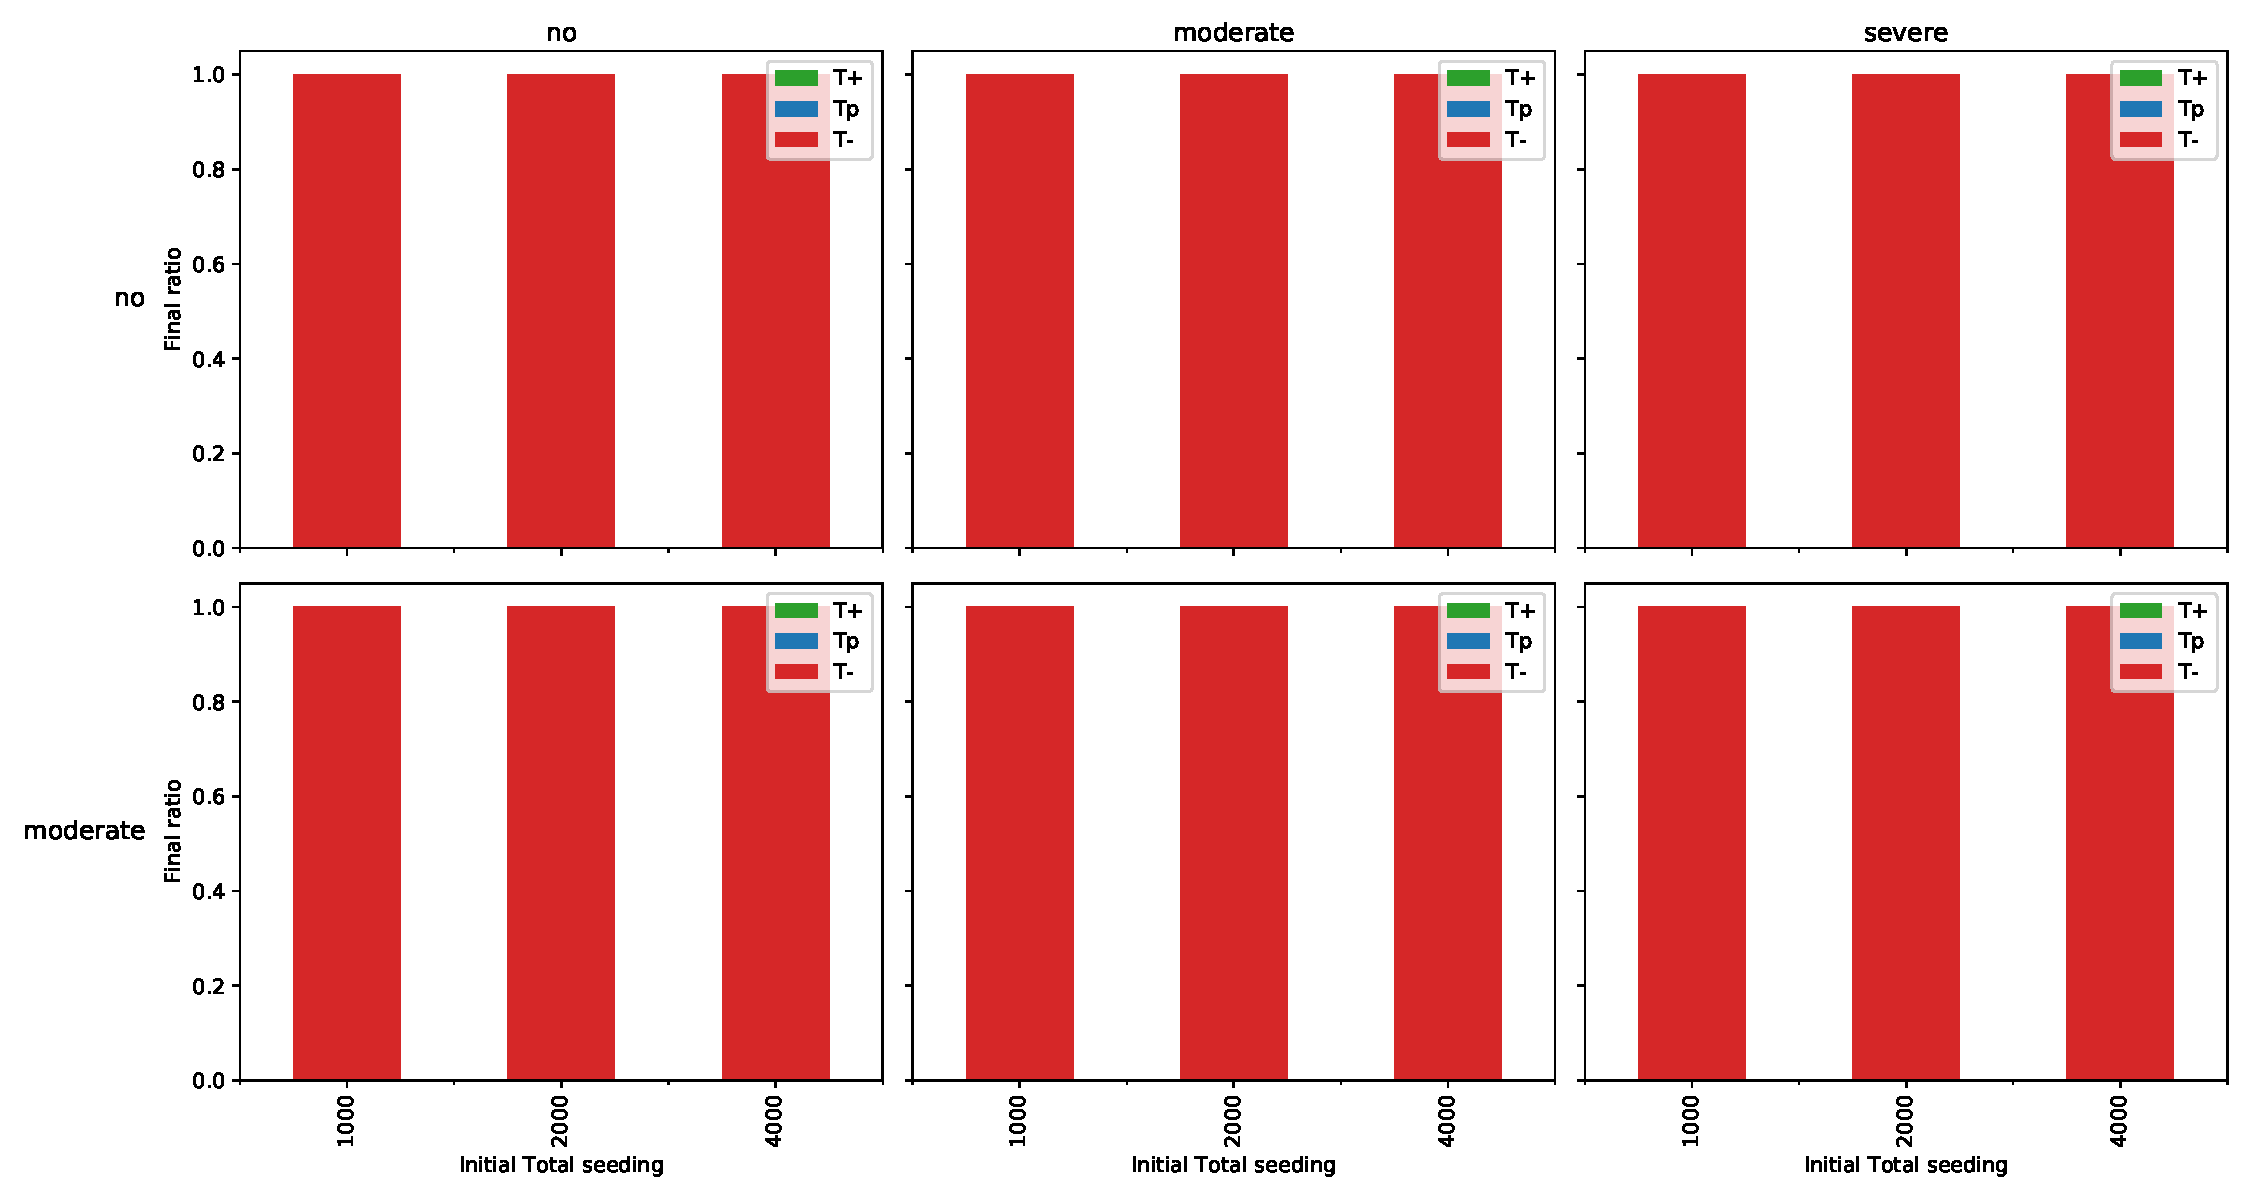
\includegraphics[width=\textwidth]{All3_therapy-SOC_1:1:1}
      \caption{Equal seeding - 1:1:1}
    \end{subfigure}
    \begin{subfigure}[b]{0.48\textwidth}
      \centering
      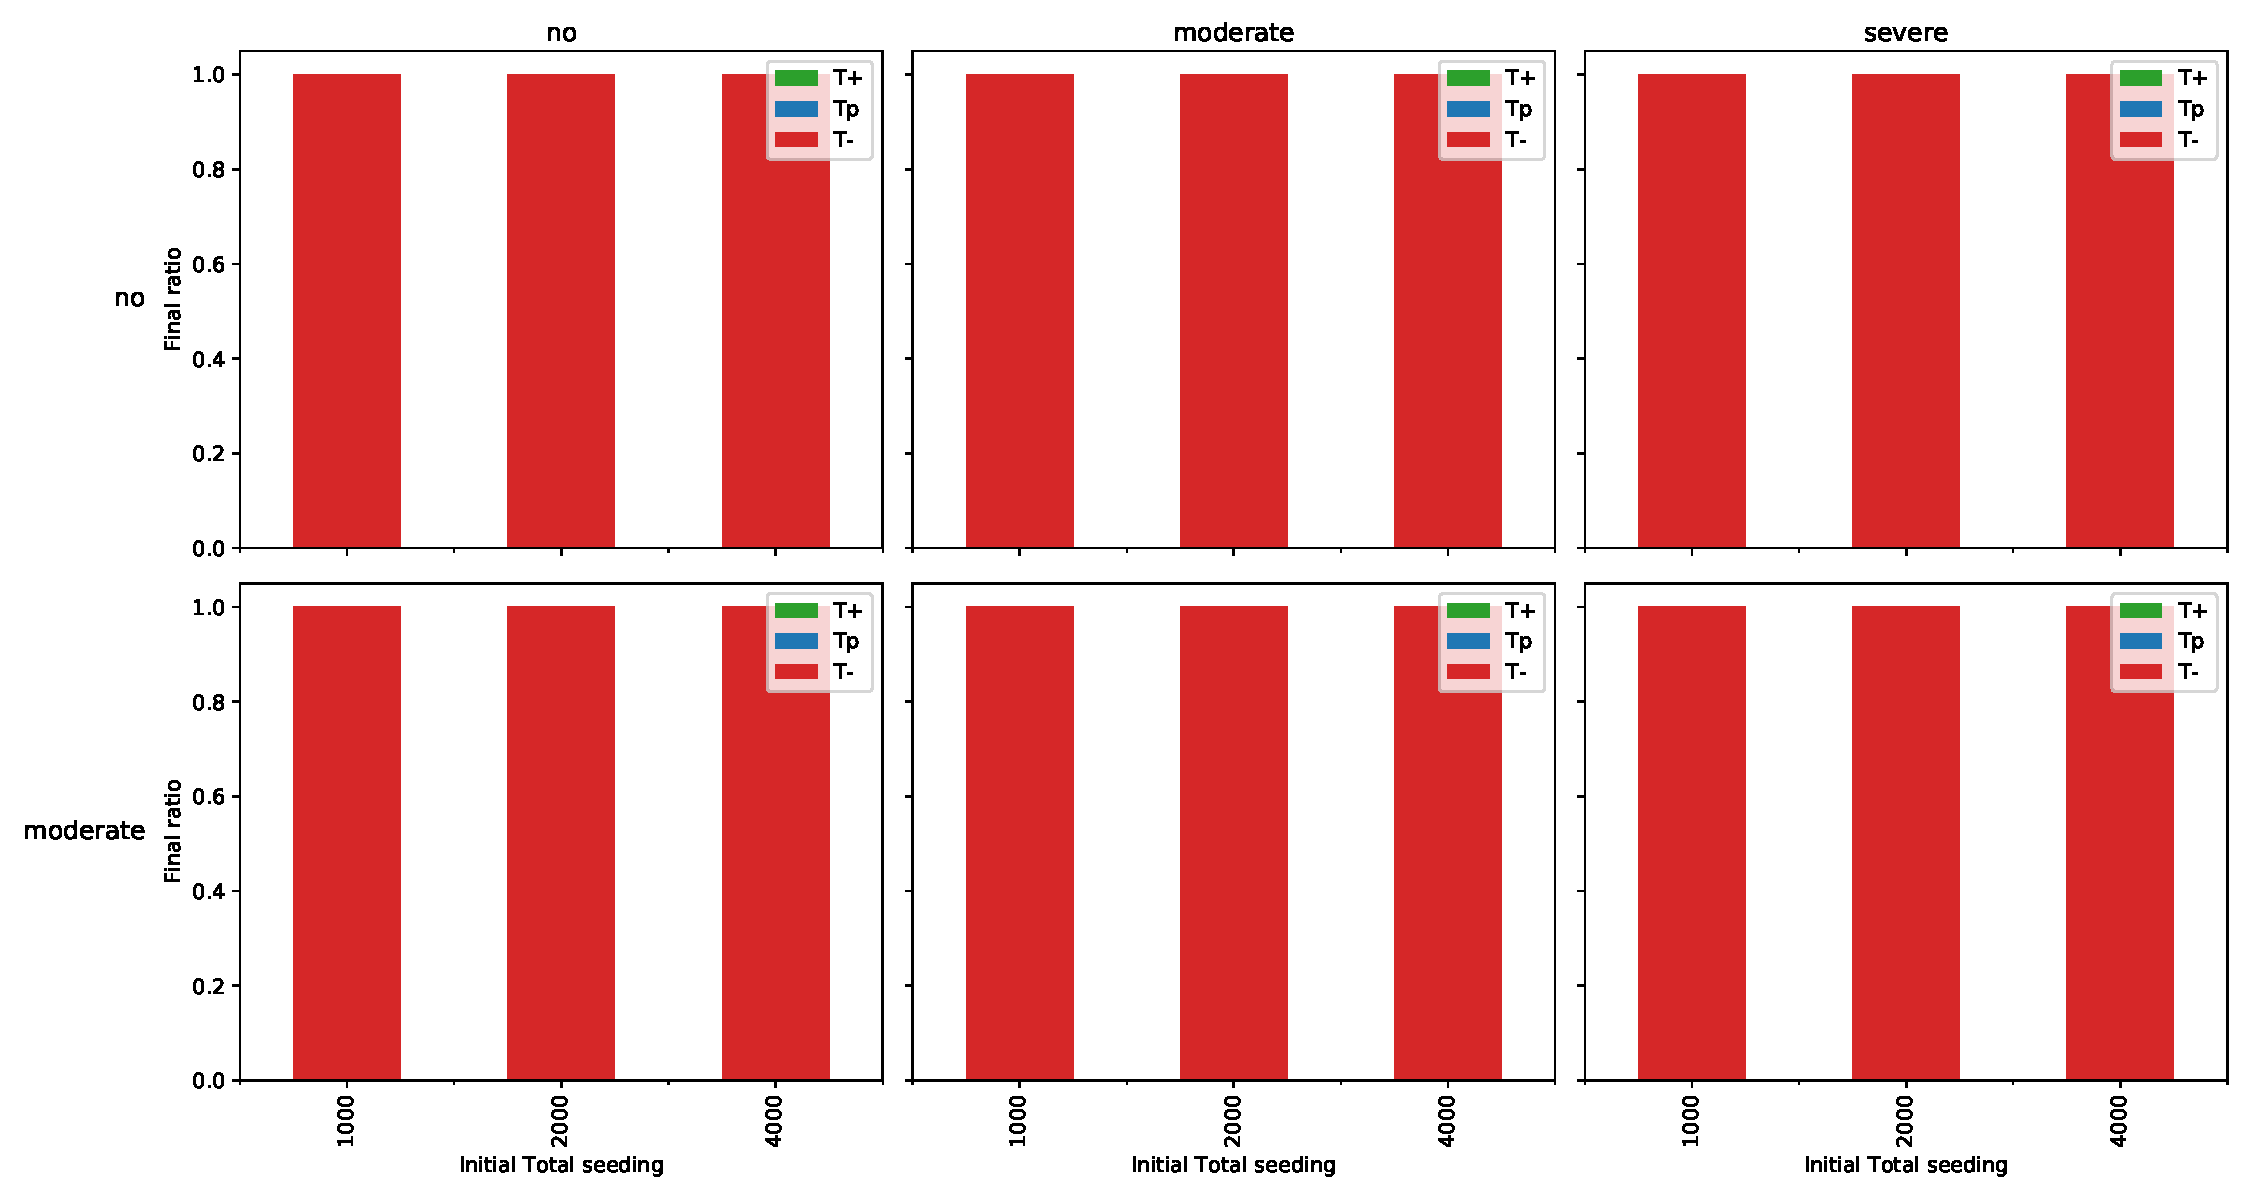
\includegraphics[width=\textwidth]{All3_therapy-SOC_8:1:1}
      \caption{High $T^p$ seeding - 8:1:1}
    \end{subfigure}
    \caption{Final ratio of all cell types under standard-of-care. C: $O_2$ limits , R: $test$ limits and SF: seeding propn. }
  \end{figure}
  \begin{columns}
    \begin{column}{0.5\textwidth}
      \begin{itemize}
        \item $T^+, T^p$ extinct: all cases
      \end{itemize}
    \end{column}
    \begin{column}{0.5\textwidth}
      \begin{itemize}
        \item $test$: insufficient
      \end{itemize}
    \end{column}
  \end{columns}
\end{frame}

\begin{frame}{Adaptive Therapy (AT) thresholds}
  \begin{figure}[h]
    \centering
    \begin{subfigure}[b]{0.48\textwidth}
      \centering
      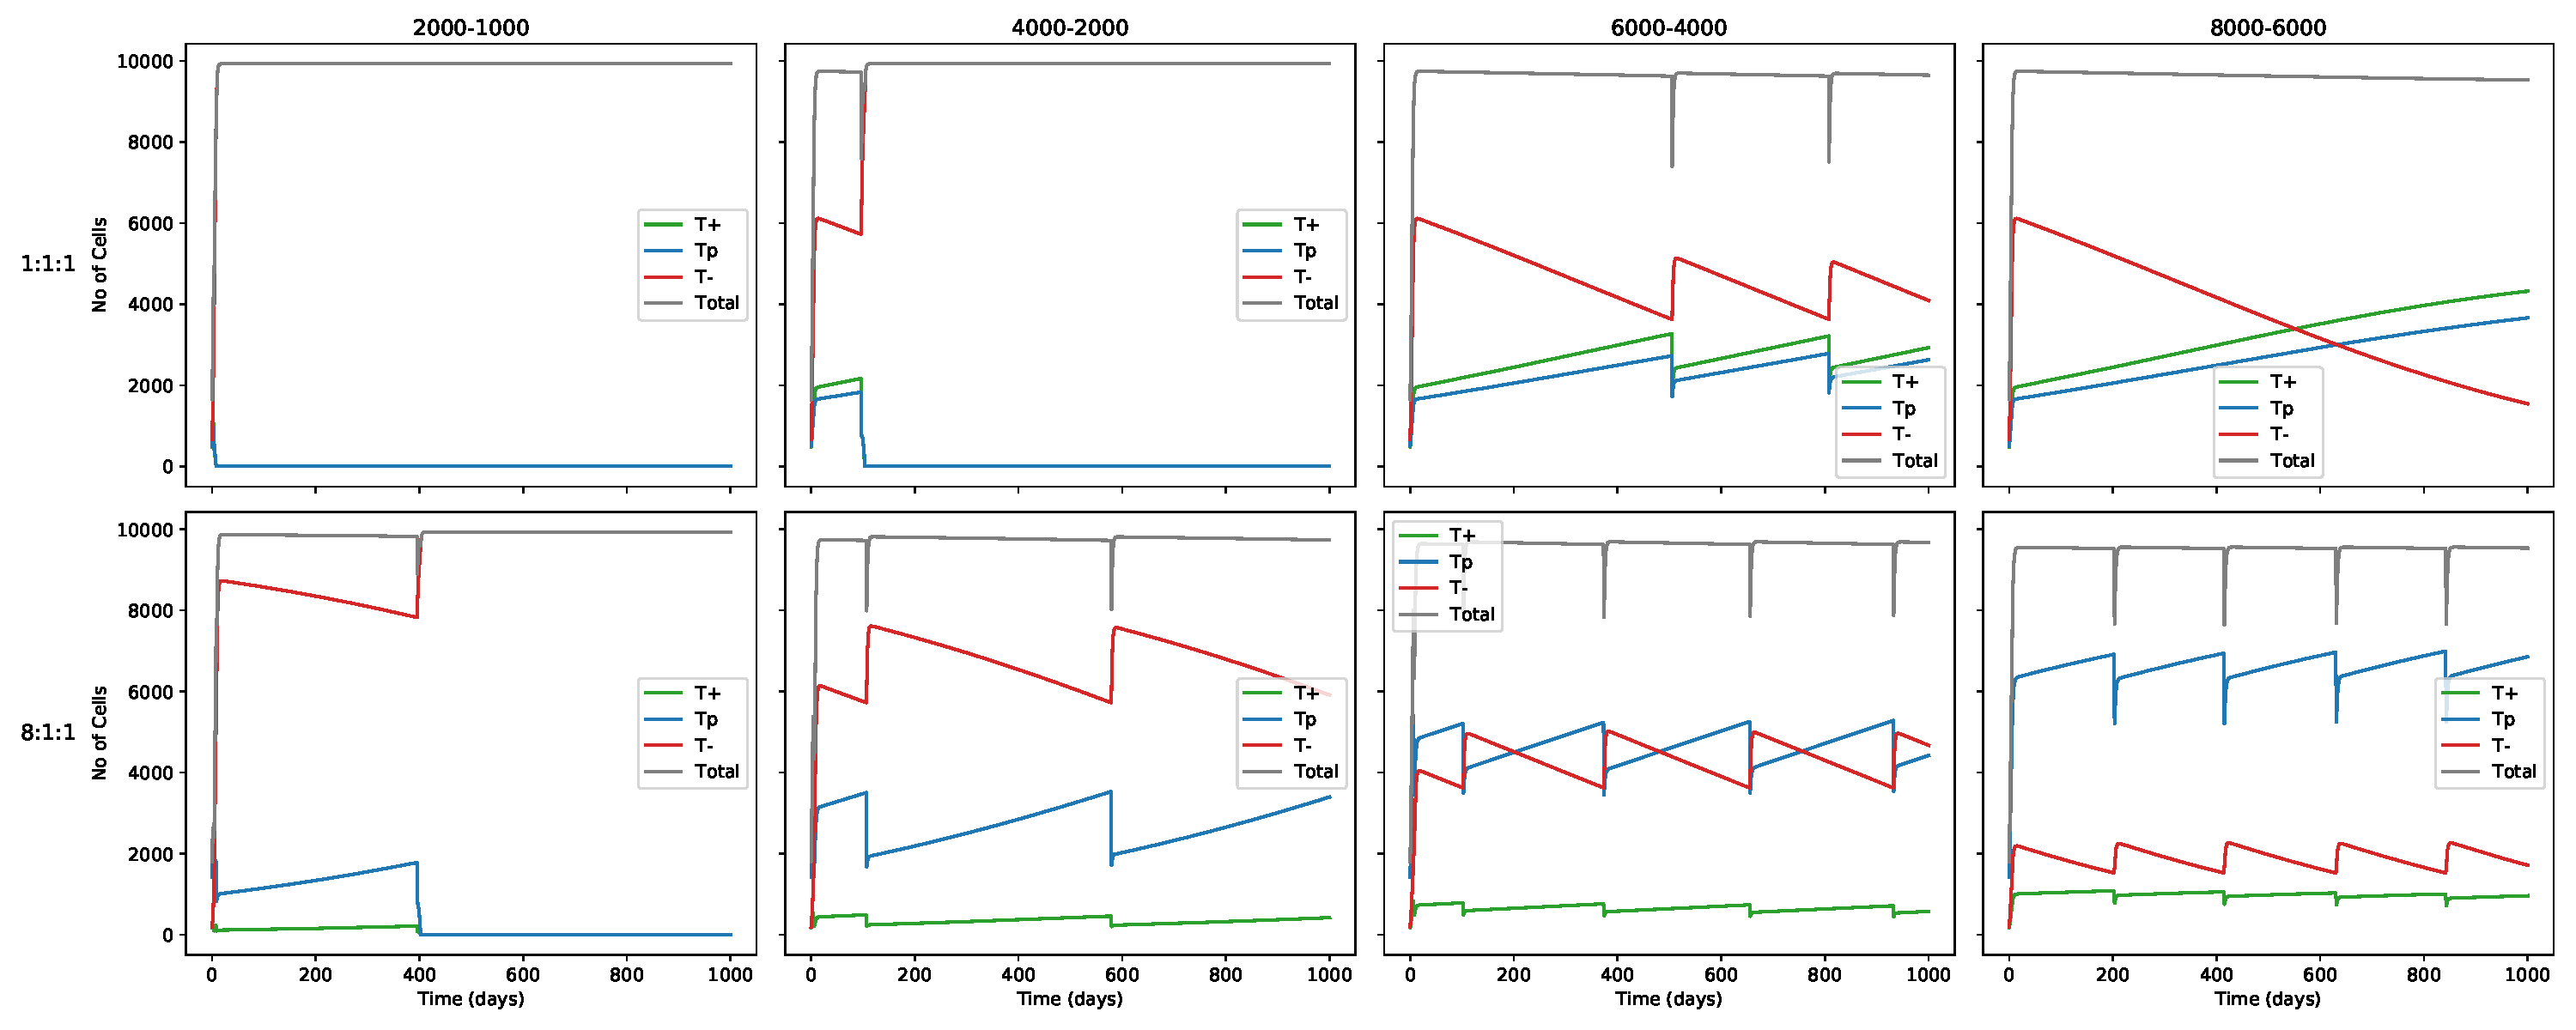
\includegraphics[width=\textwidth]{All3_therapy-standardization}
    \end{subfigure}
    \begin{subfigure}[b]{0.48\textwidth}
      \centering
      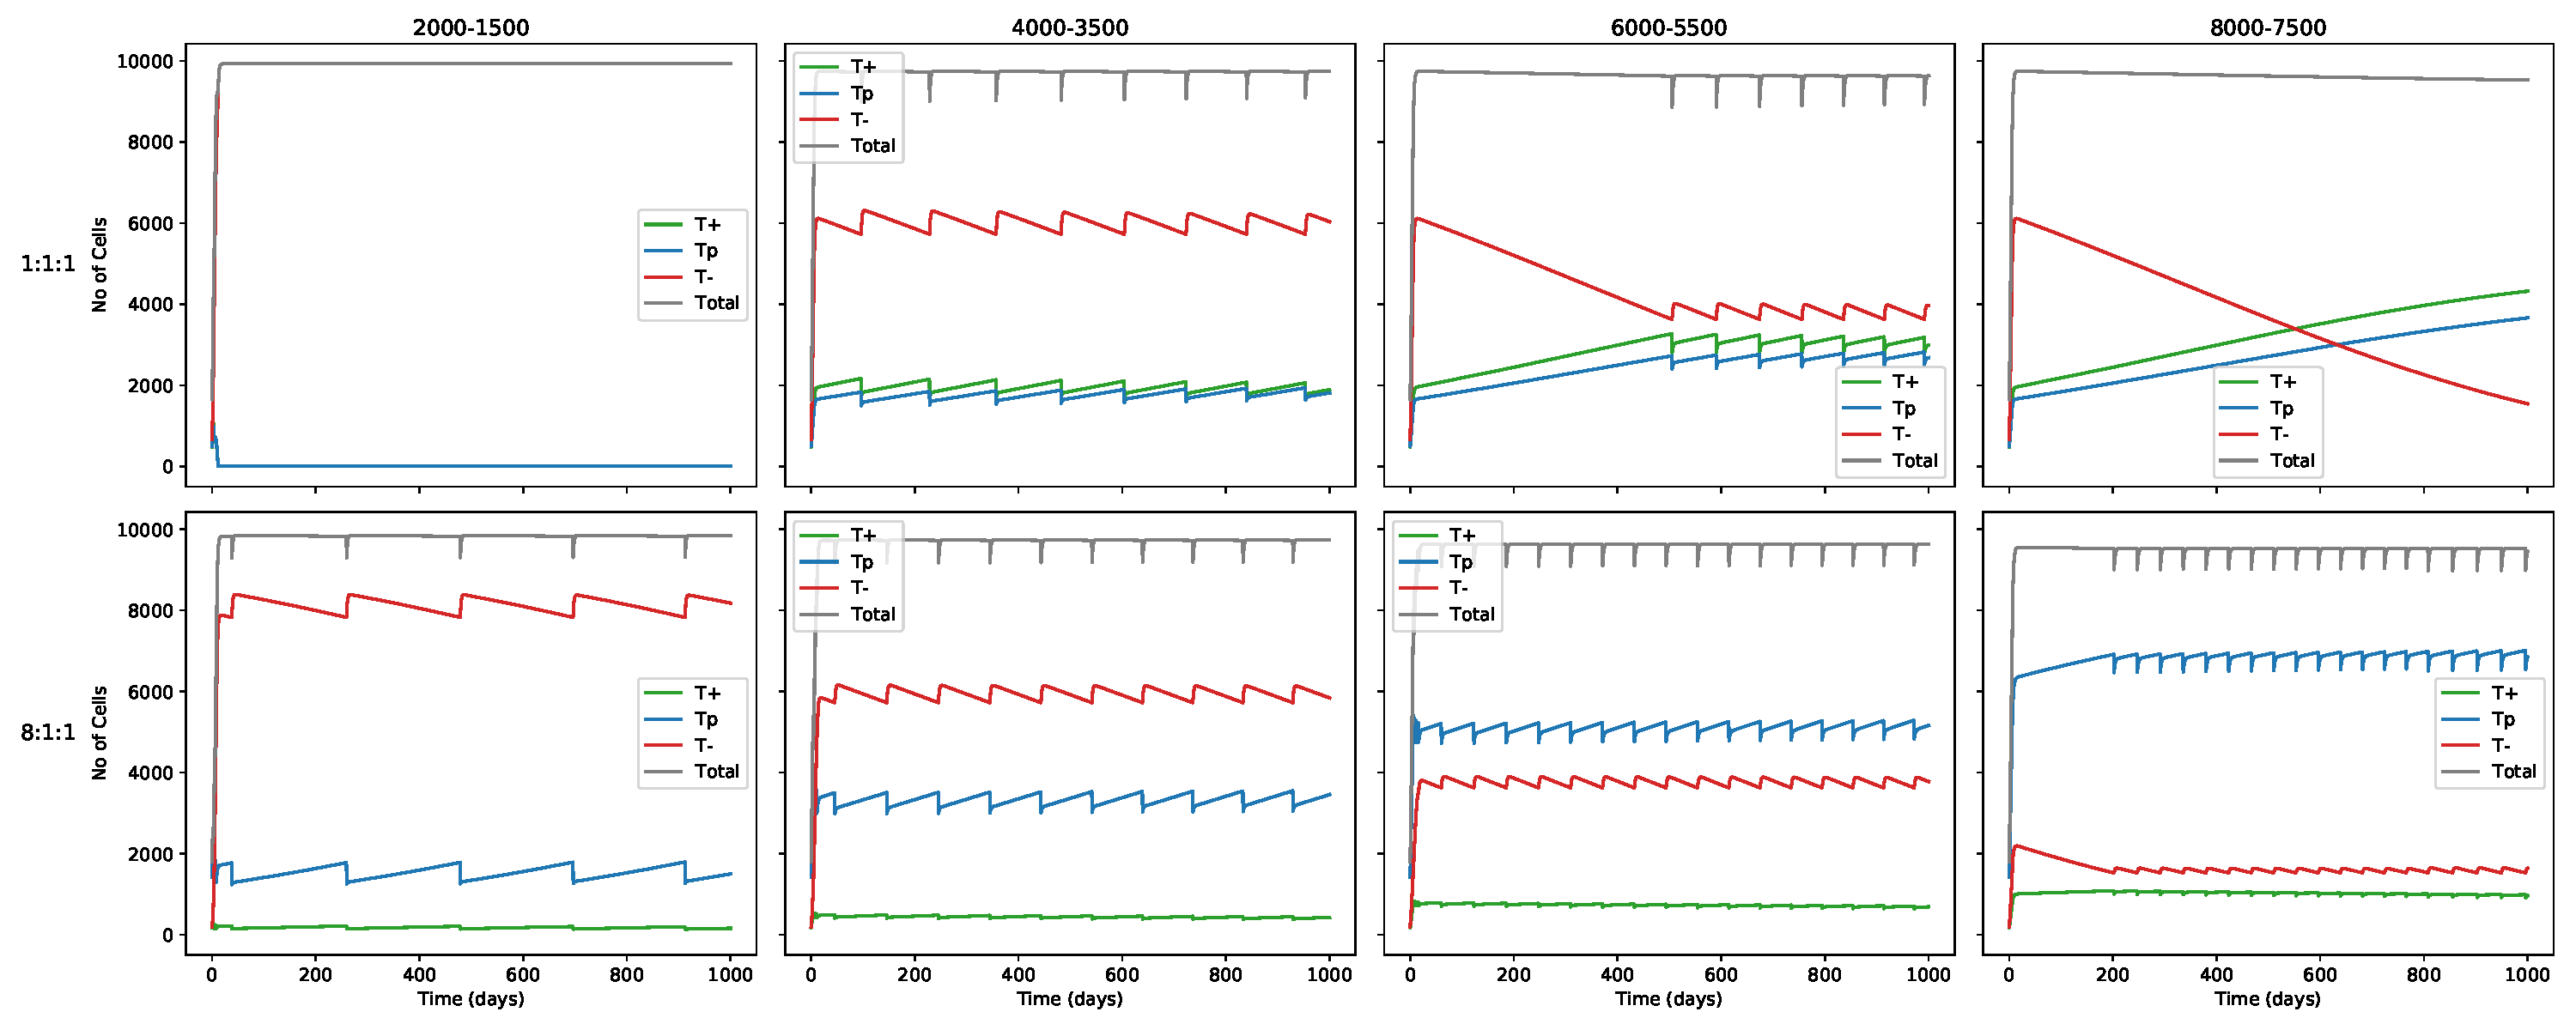
\includegraphics[width=\textwidth]{All3_therapy-standardization-sw}
    \end{subfigure}
    \caption{Standardisation of threshold for AT, C: On-Off threshold, R: $T^p:T^+:T^-$ Seeding}
  \end{figure}
  \begin{columns}
    \begin{column}{0.5\textwidth}
      \begin{itemize}
        \item $50\%$ rule
        \item Low threshold: $T^-$ inhibits
        \item High threshold: better \cite{Hansen}
      \end{itemize}
    \end{column}
    \begin{column}{0.5\textwidth}
      \begin{itemize}
        \item Too high: no therapy
        \item On: 6000, Off: 4000
        \item Popn. size $T^+ - T^p$
      \end{itemize}
    \end{column}
  \end{columns}
\end{frame}

\begin{frame}{AT}
  \begin{figure}[h]
    \centering
    \begin{subfigure}[b]{0.48\textwidth}
      \centering
      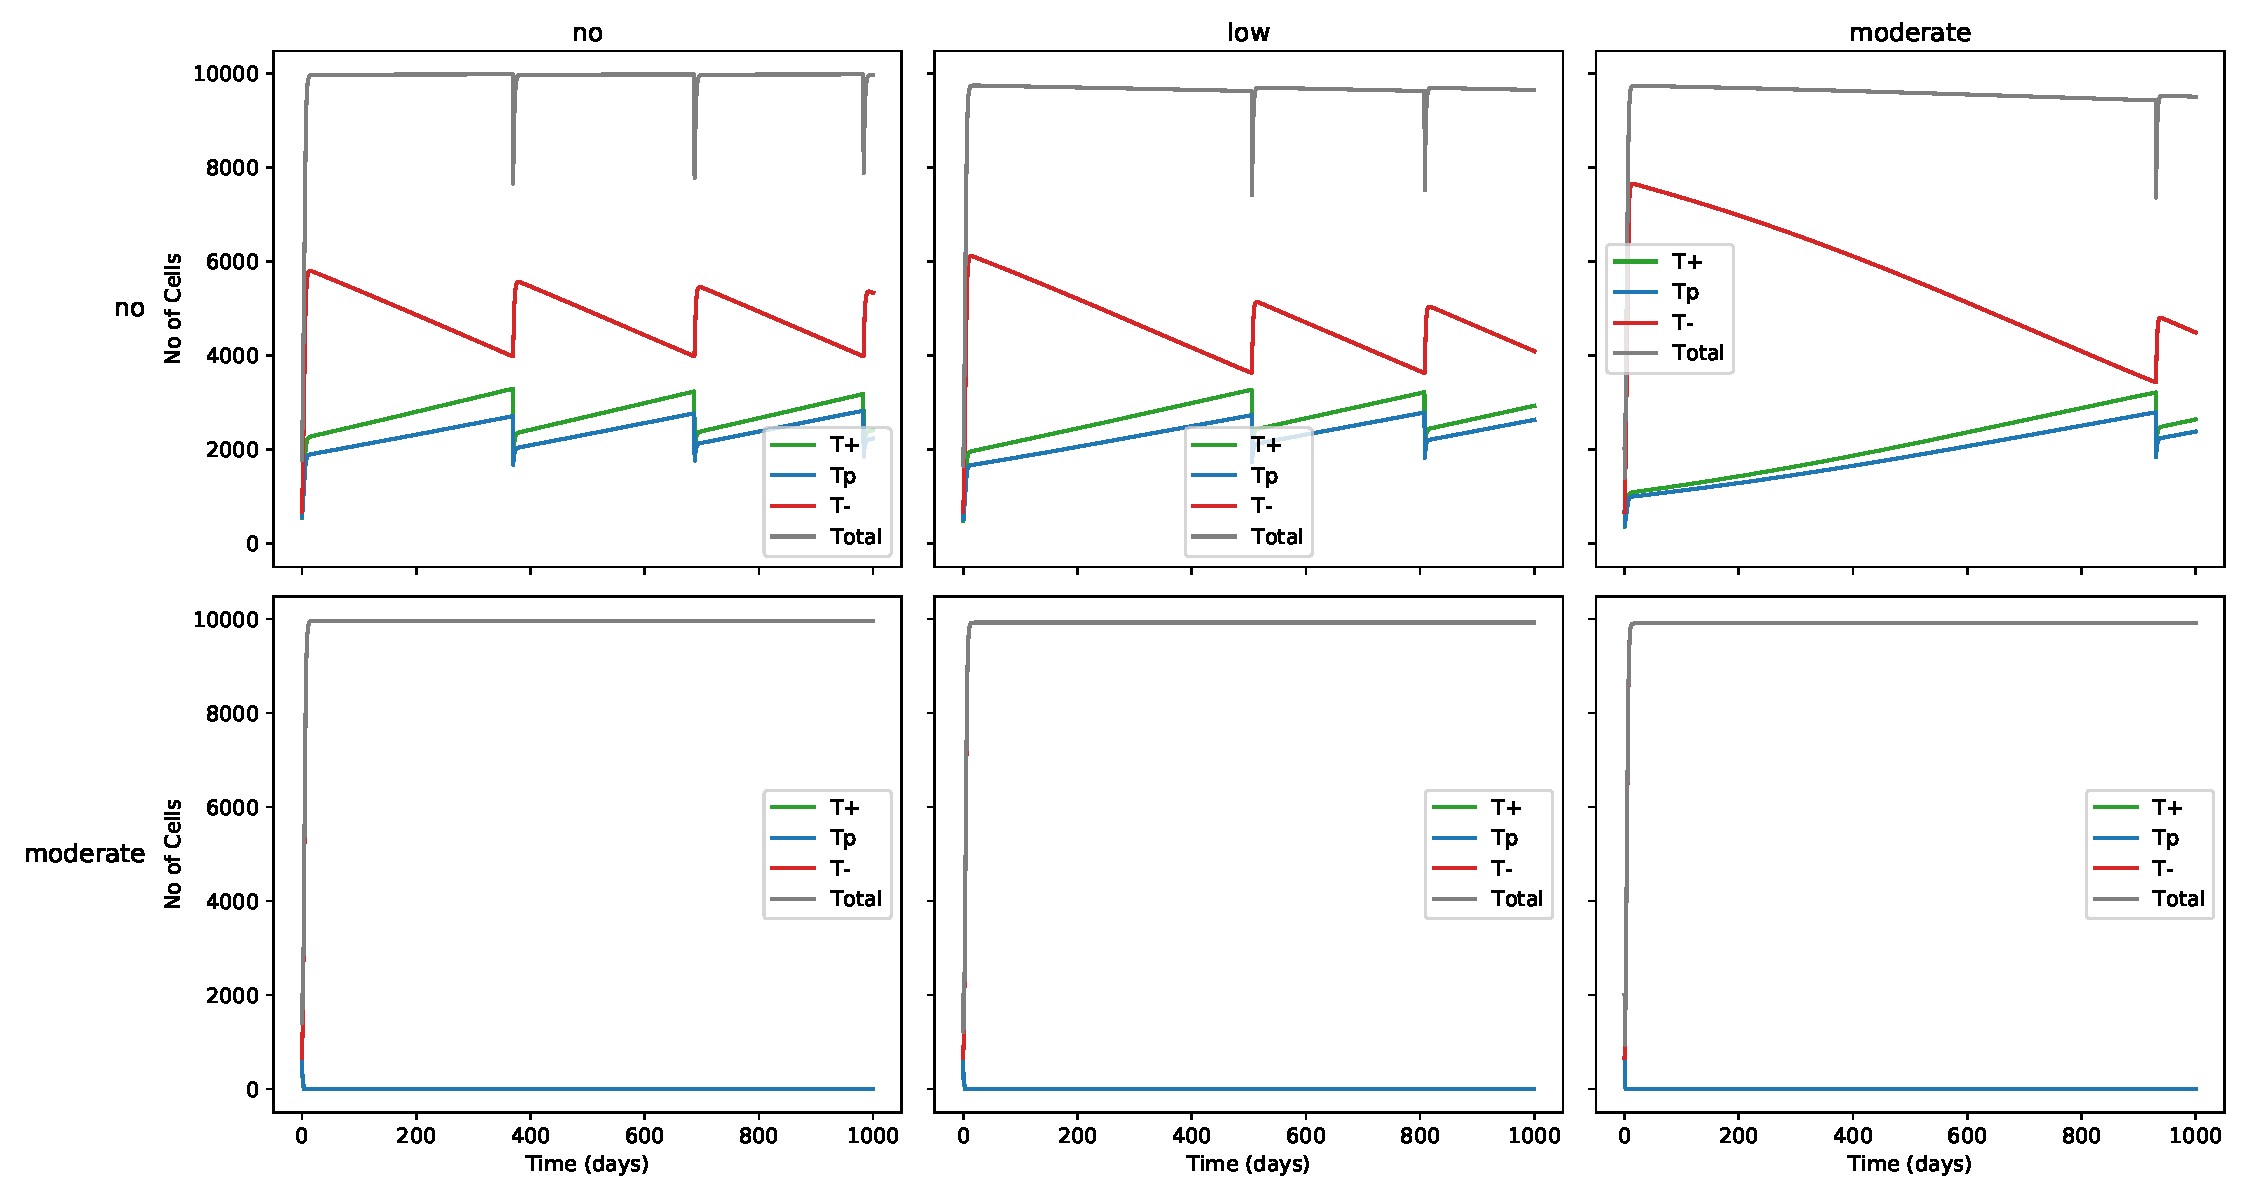
\includegraphics[width=\textwidth]{All3_therapy_1:1:1-2000}
      \caption{Equal seeding - 1:1:1}
    \end{subfigure}
    \begin{subfigure}[b]{0.48\textwidth}
      \centering
      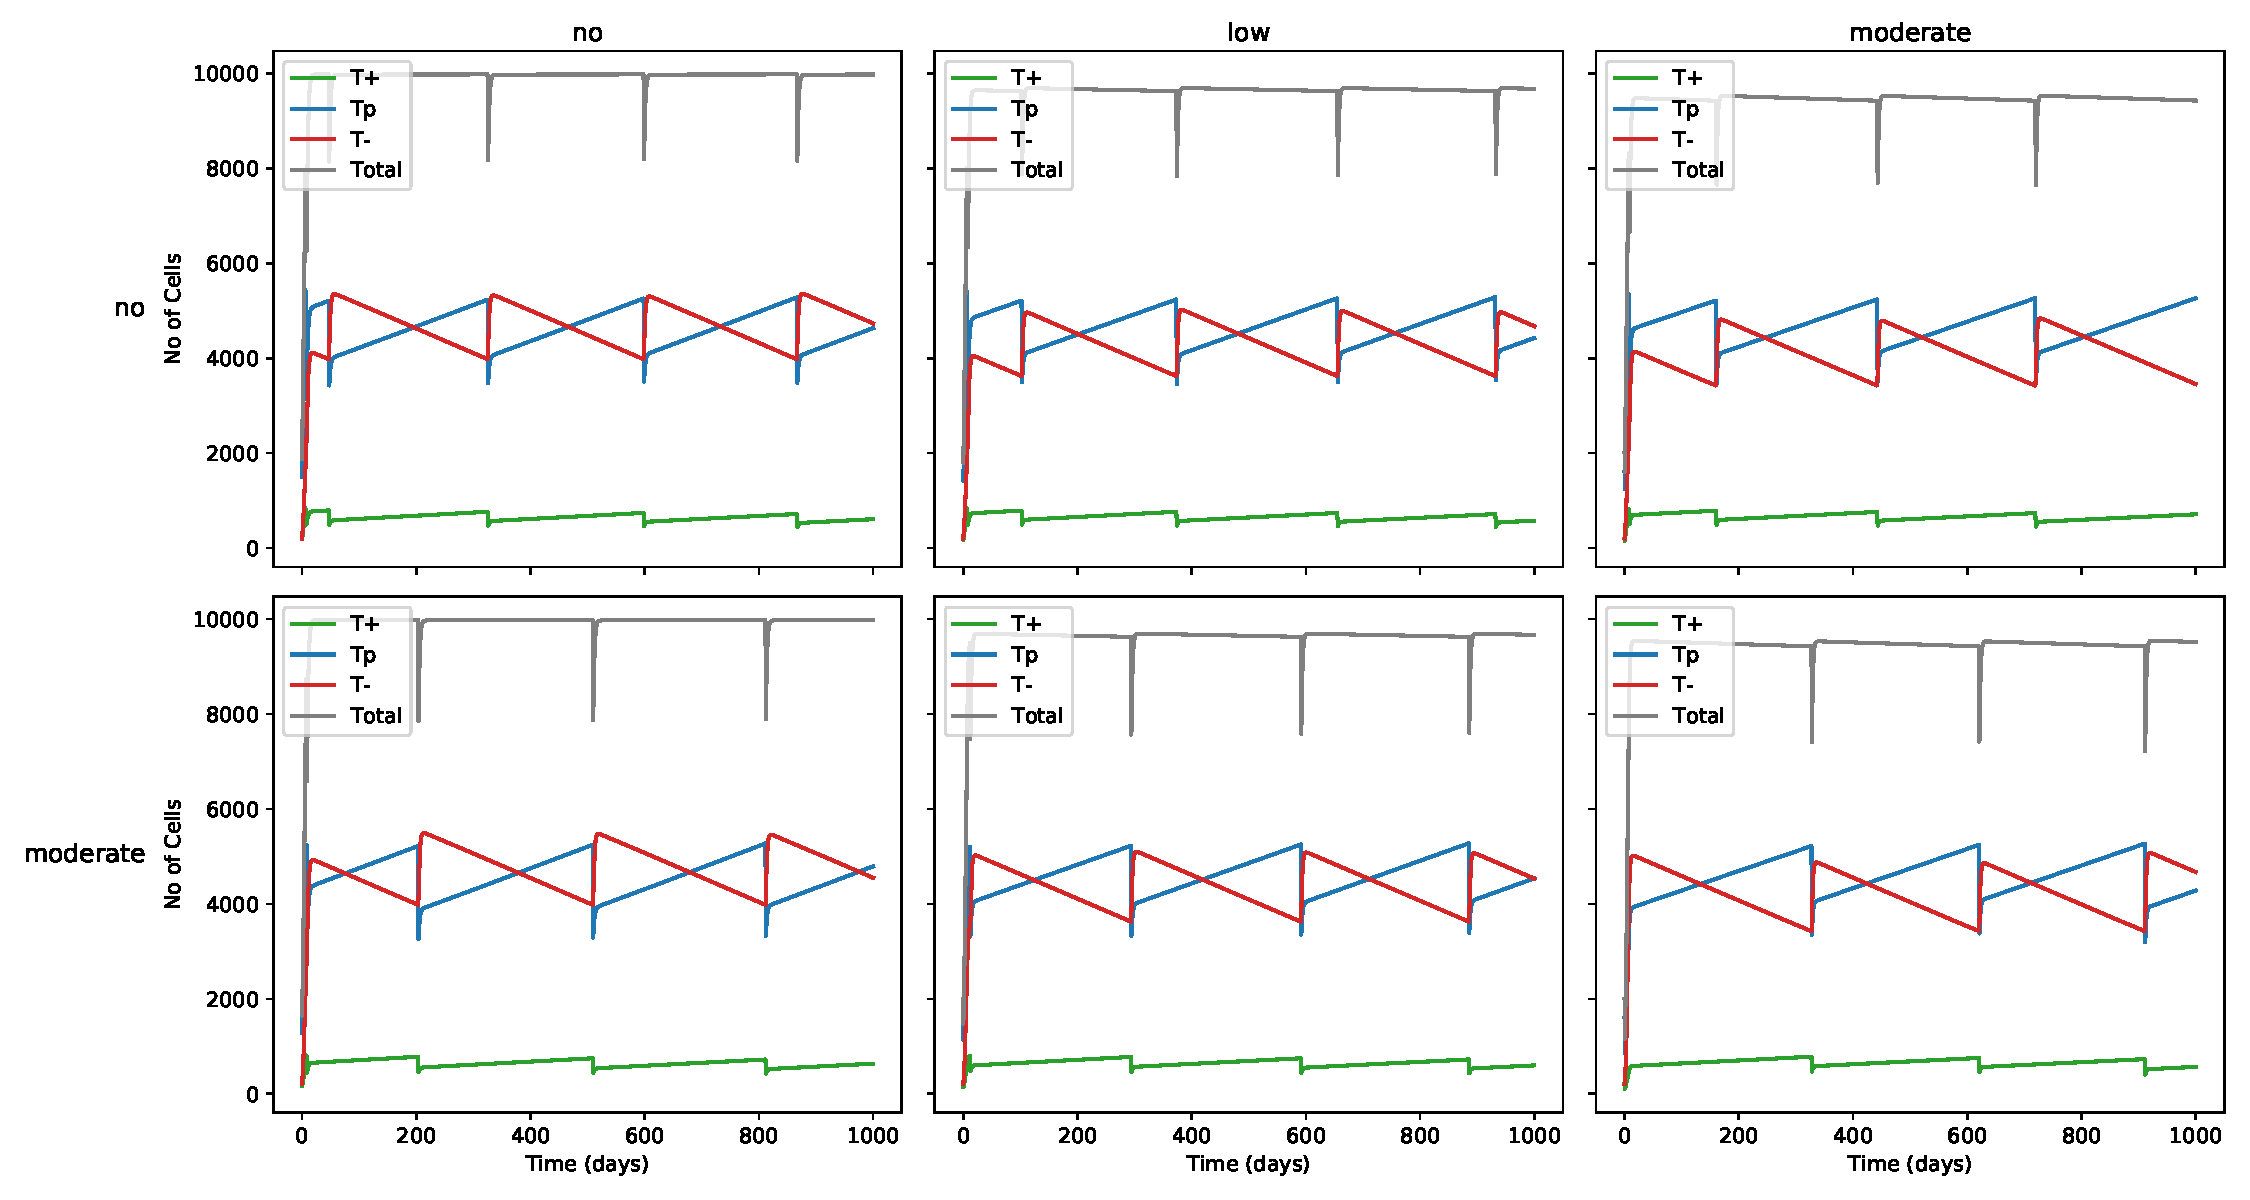
\includegraphics[width=\textwidth]{All3_therapy_8:1:1-2000}
      \caption{High $T^p$ seeding - 8:1:1}
    \end{subfigure}
    \caption{Time-series of all cell types with AT. C: $O_2$ limits, R: $test$ limits and SF: seeding propn. (On:6000, Off:4000)}
  \end{figure}
  \begin{columns}
    \begin{column}{0.5\textwidth}
      \begin{itemize}
        \item Higher $T^+ - T^p$: more treatable
        \item $test$ mod.: extinct from comp.
      \end{itemize}
    \end{column}
    \begin{column}{0.5\textwidth}
      \begin{itemize}
        \item Apply therapy - $T^-$ quickly replace \\
        $\rightarrow$ tot. popn. high
      \end{itemize}
    \end{column}
  \end{columns}
\end{frame}

\begin{frame}{AT w/ delay}
  \begin{figure}[h]
    \centering
    \begin{subfigure}[b]{0.48\textwidth}
      \centering
      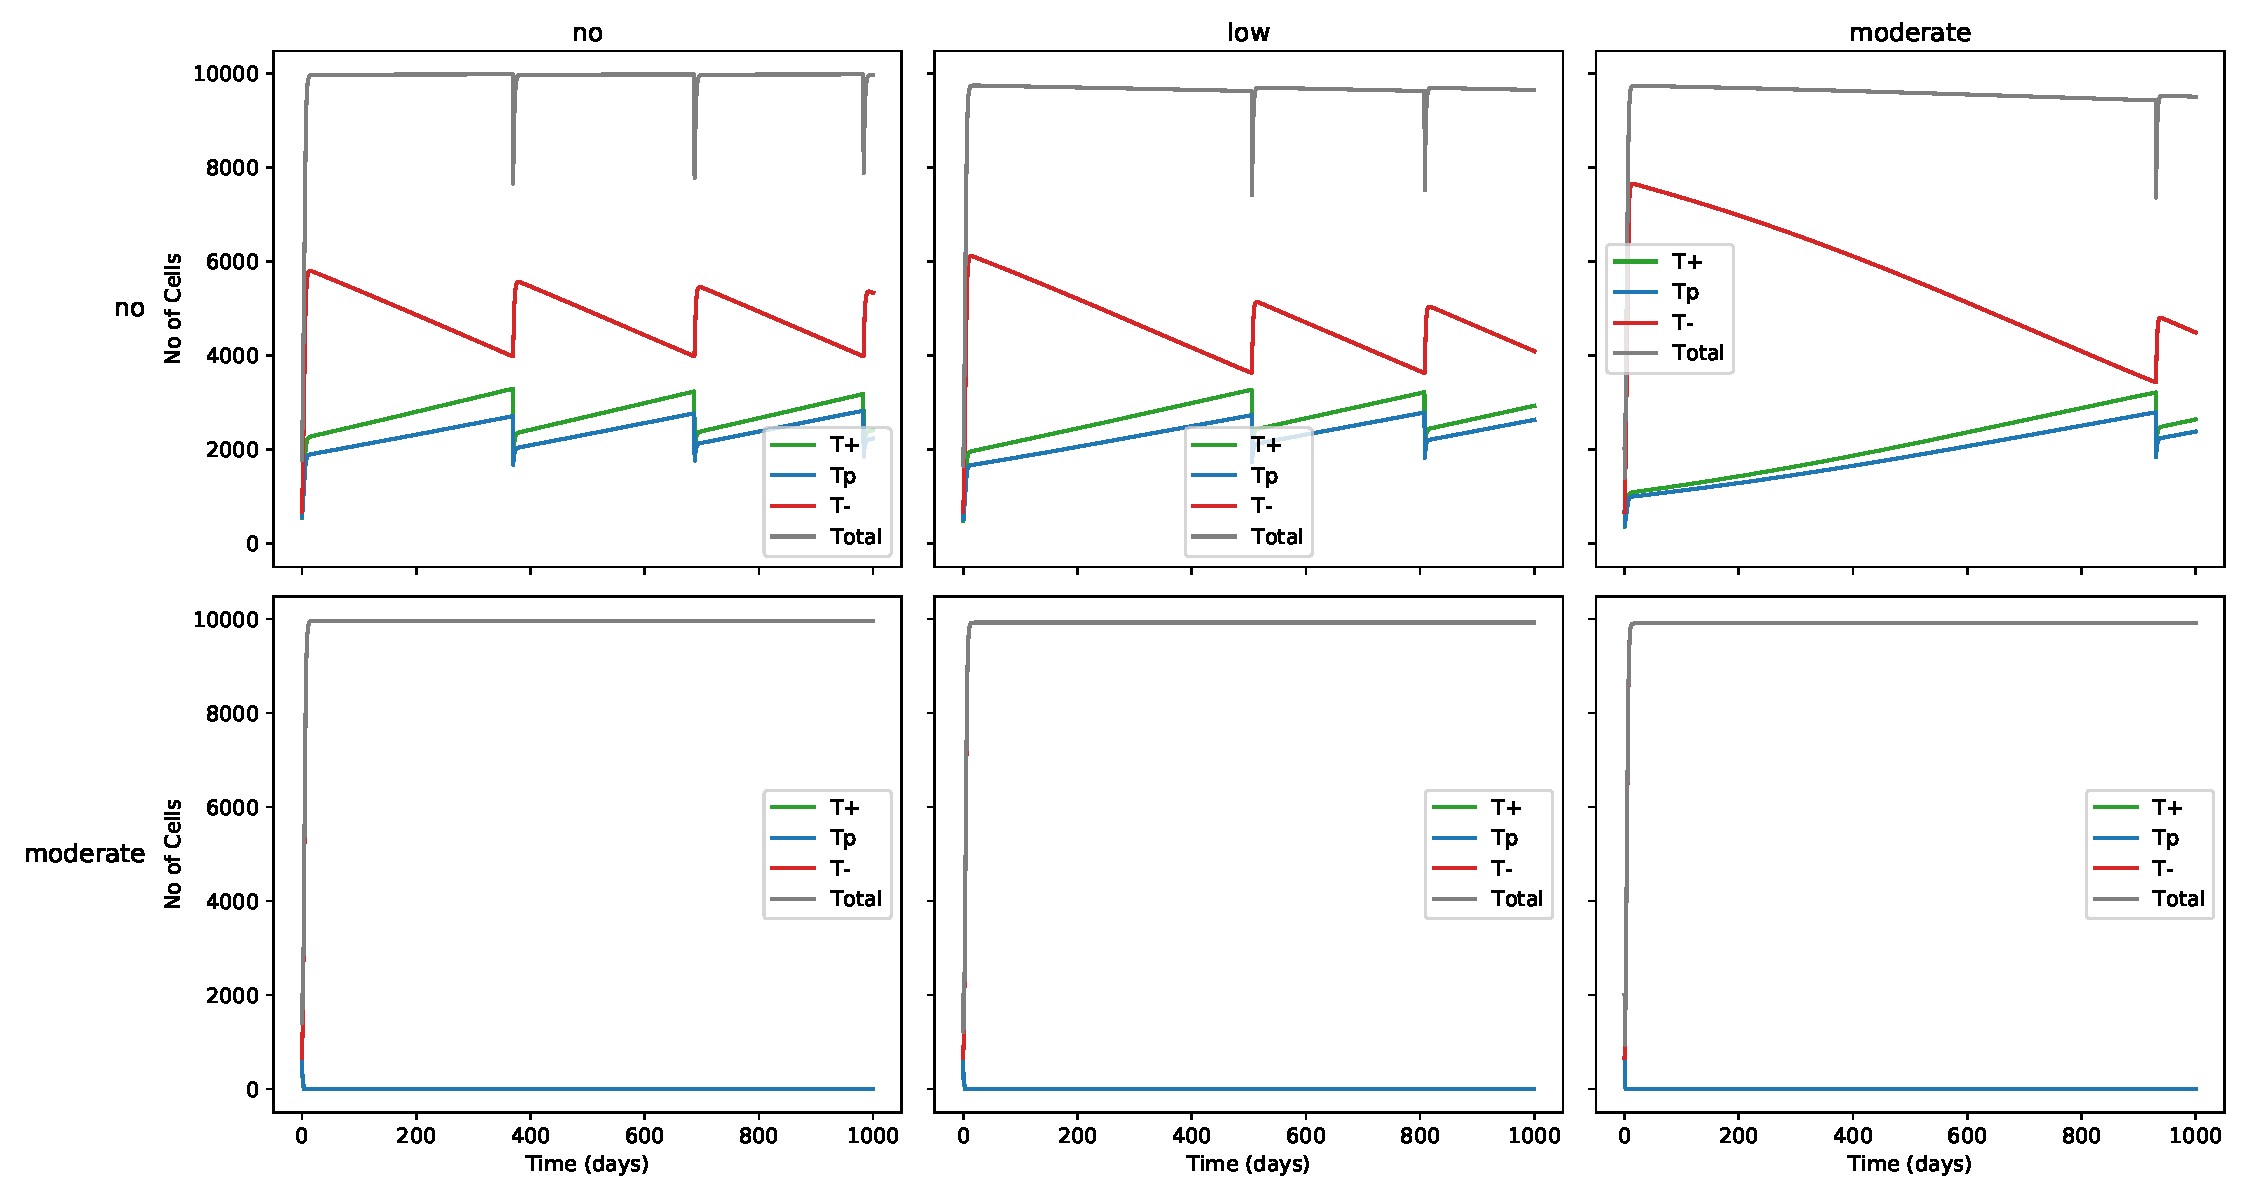
\includegraphics[width=\textwidth]{All3_therapy_200day_1:1:1}
      \caption{Equal seeding - 1:1:1}
    \end{subfigure}
    \begin{subfigure}[b]{0.48\textwidth}
      \centering
      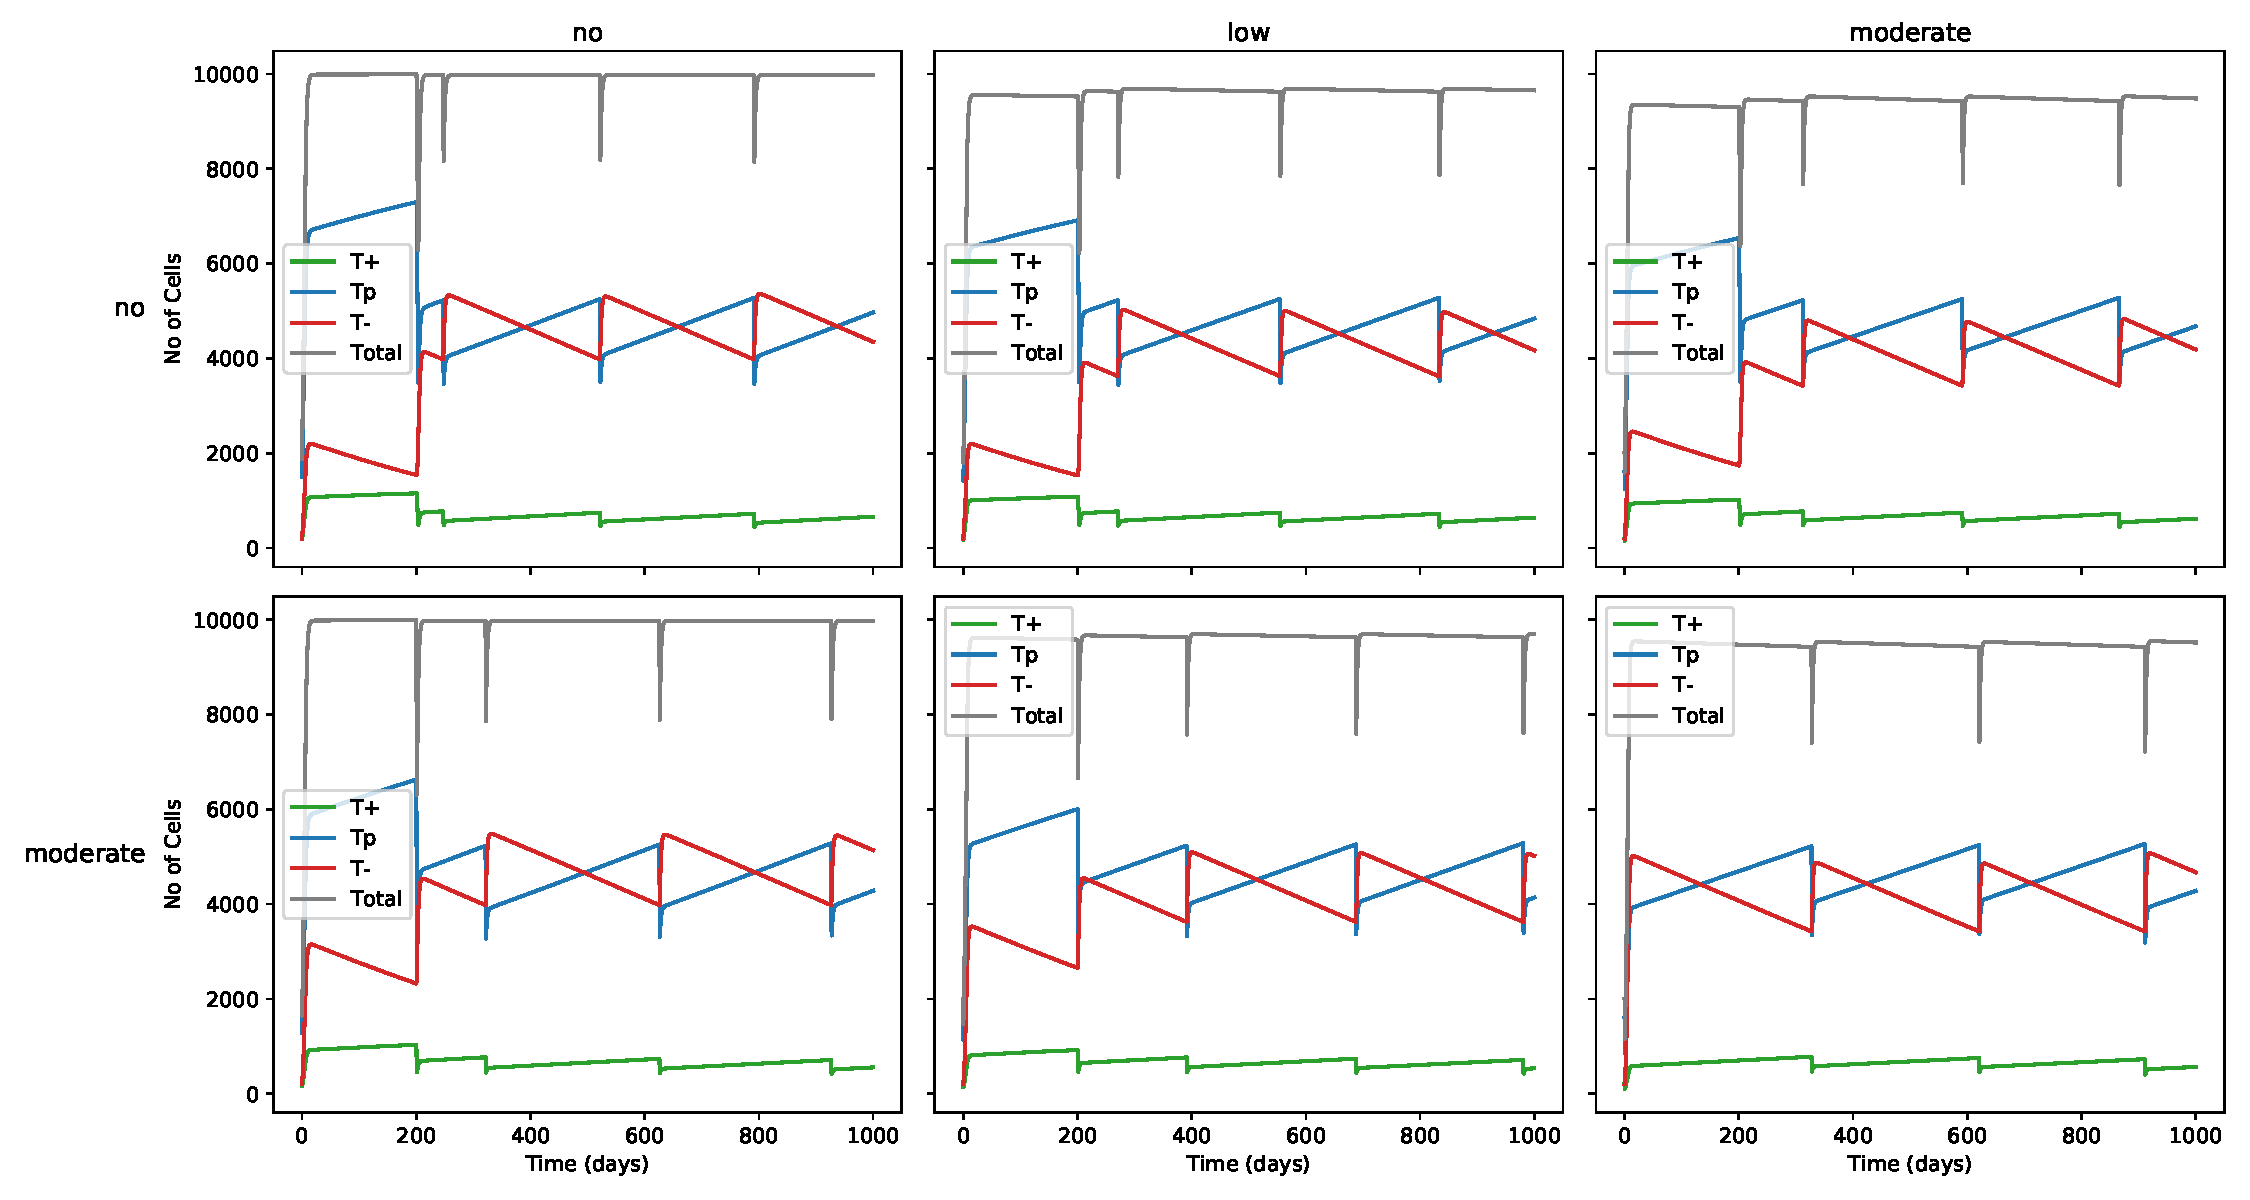
\includegraphics[width=\textwidth]{All3_therapy_200day_8:1:1}
      \caption{High $T^p$ seeding - 8:1:1}
    \end{subfigure}
    \caption{Time-series of all cell types with AT delayed by 200 days. C: $O_2$ limits, R: $test$ limits and SF: seeding propn. (On:6000, Off:4000)}
  \end{figure}
  \begin{columns}
    \begin{column}{0.5\textwidth}
      \begin{itemize}
        \item Speculate: delay $\rightarrow$ $T^+ - T^p$ $\uparrow$
      \end{itemize}
    \end{column}
    \begin{column}{0.5\textwidth}
      \begin{itemize}
        \item No advantage $\leftarrow$ no variability
        \item Physiological cost
      \end{itemize}
    \end{column}
  \end{columns}
\end{frame}

\begin{frame}{Combination AT}
  \begin{figure}[h]
    \centering
    \begin{subfigure}[b]{0.48\textwidth}
      \centering
      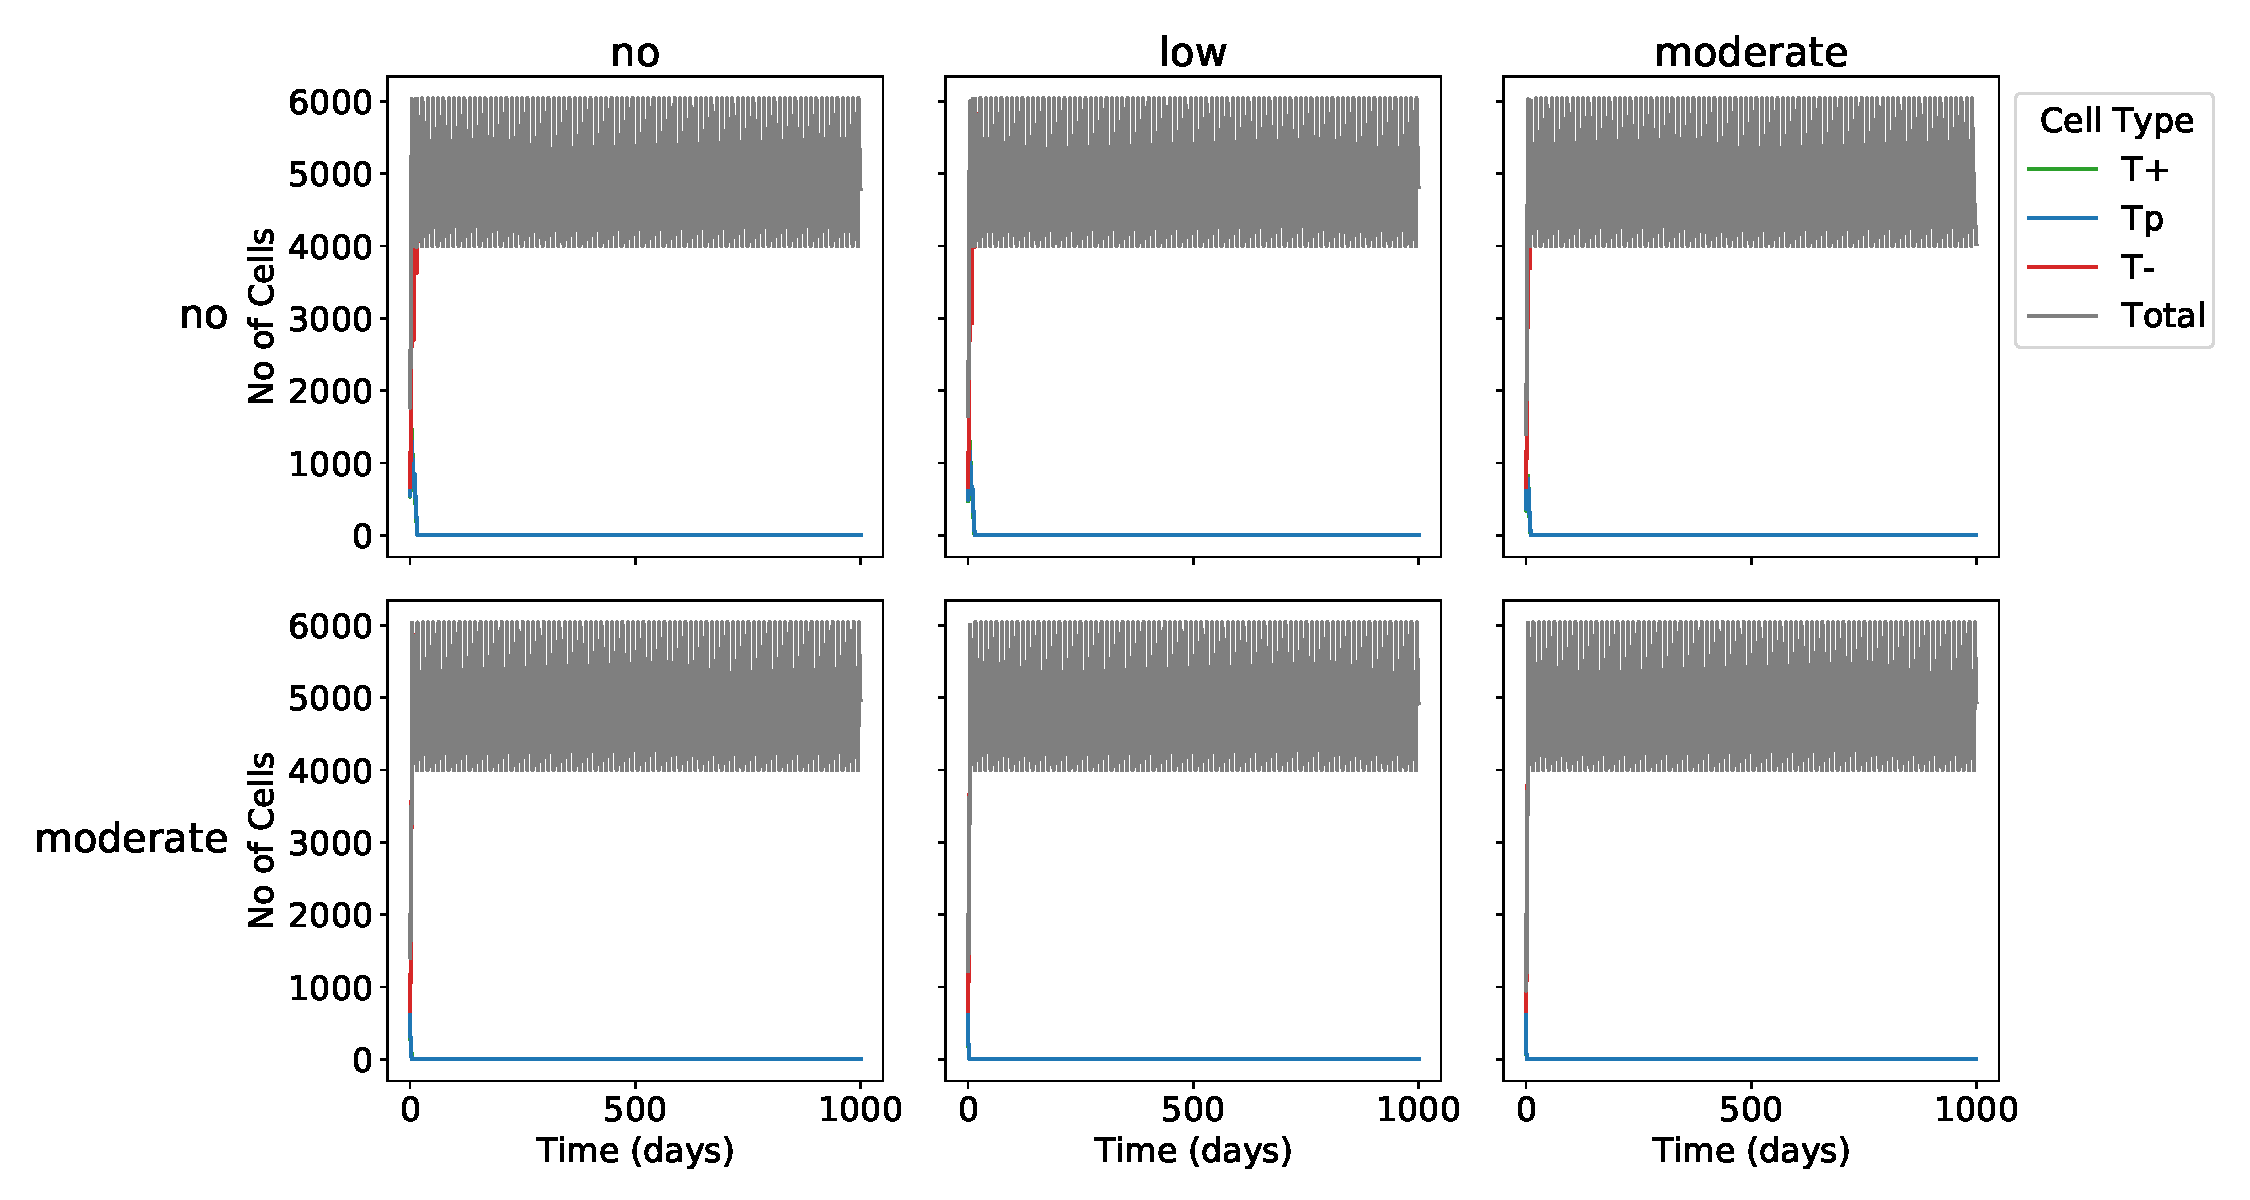
\includegraphics[width=\textwidth]{All3_therapy-combi_1:1:1}
      \caption{Equal seeding - 1:1:1}
    \end{subfigure}
    \begin{subfigure}[b]{0.48\textwidth}
      \centering
      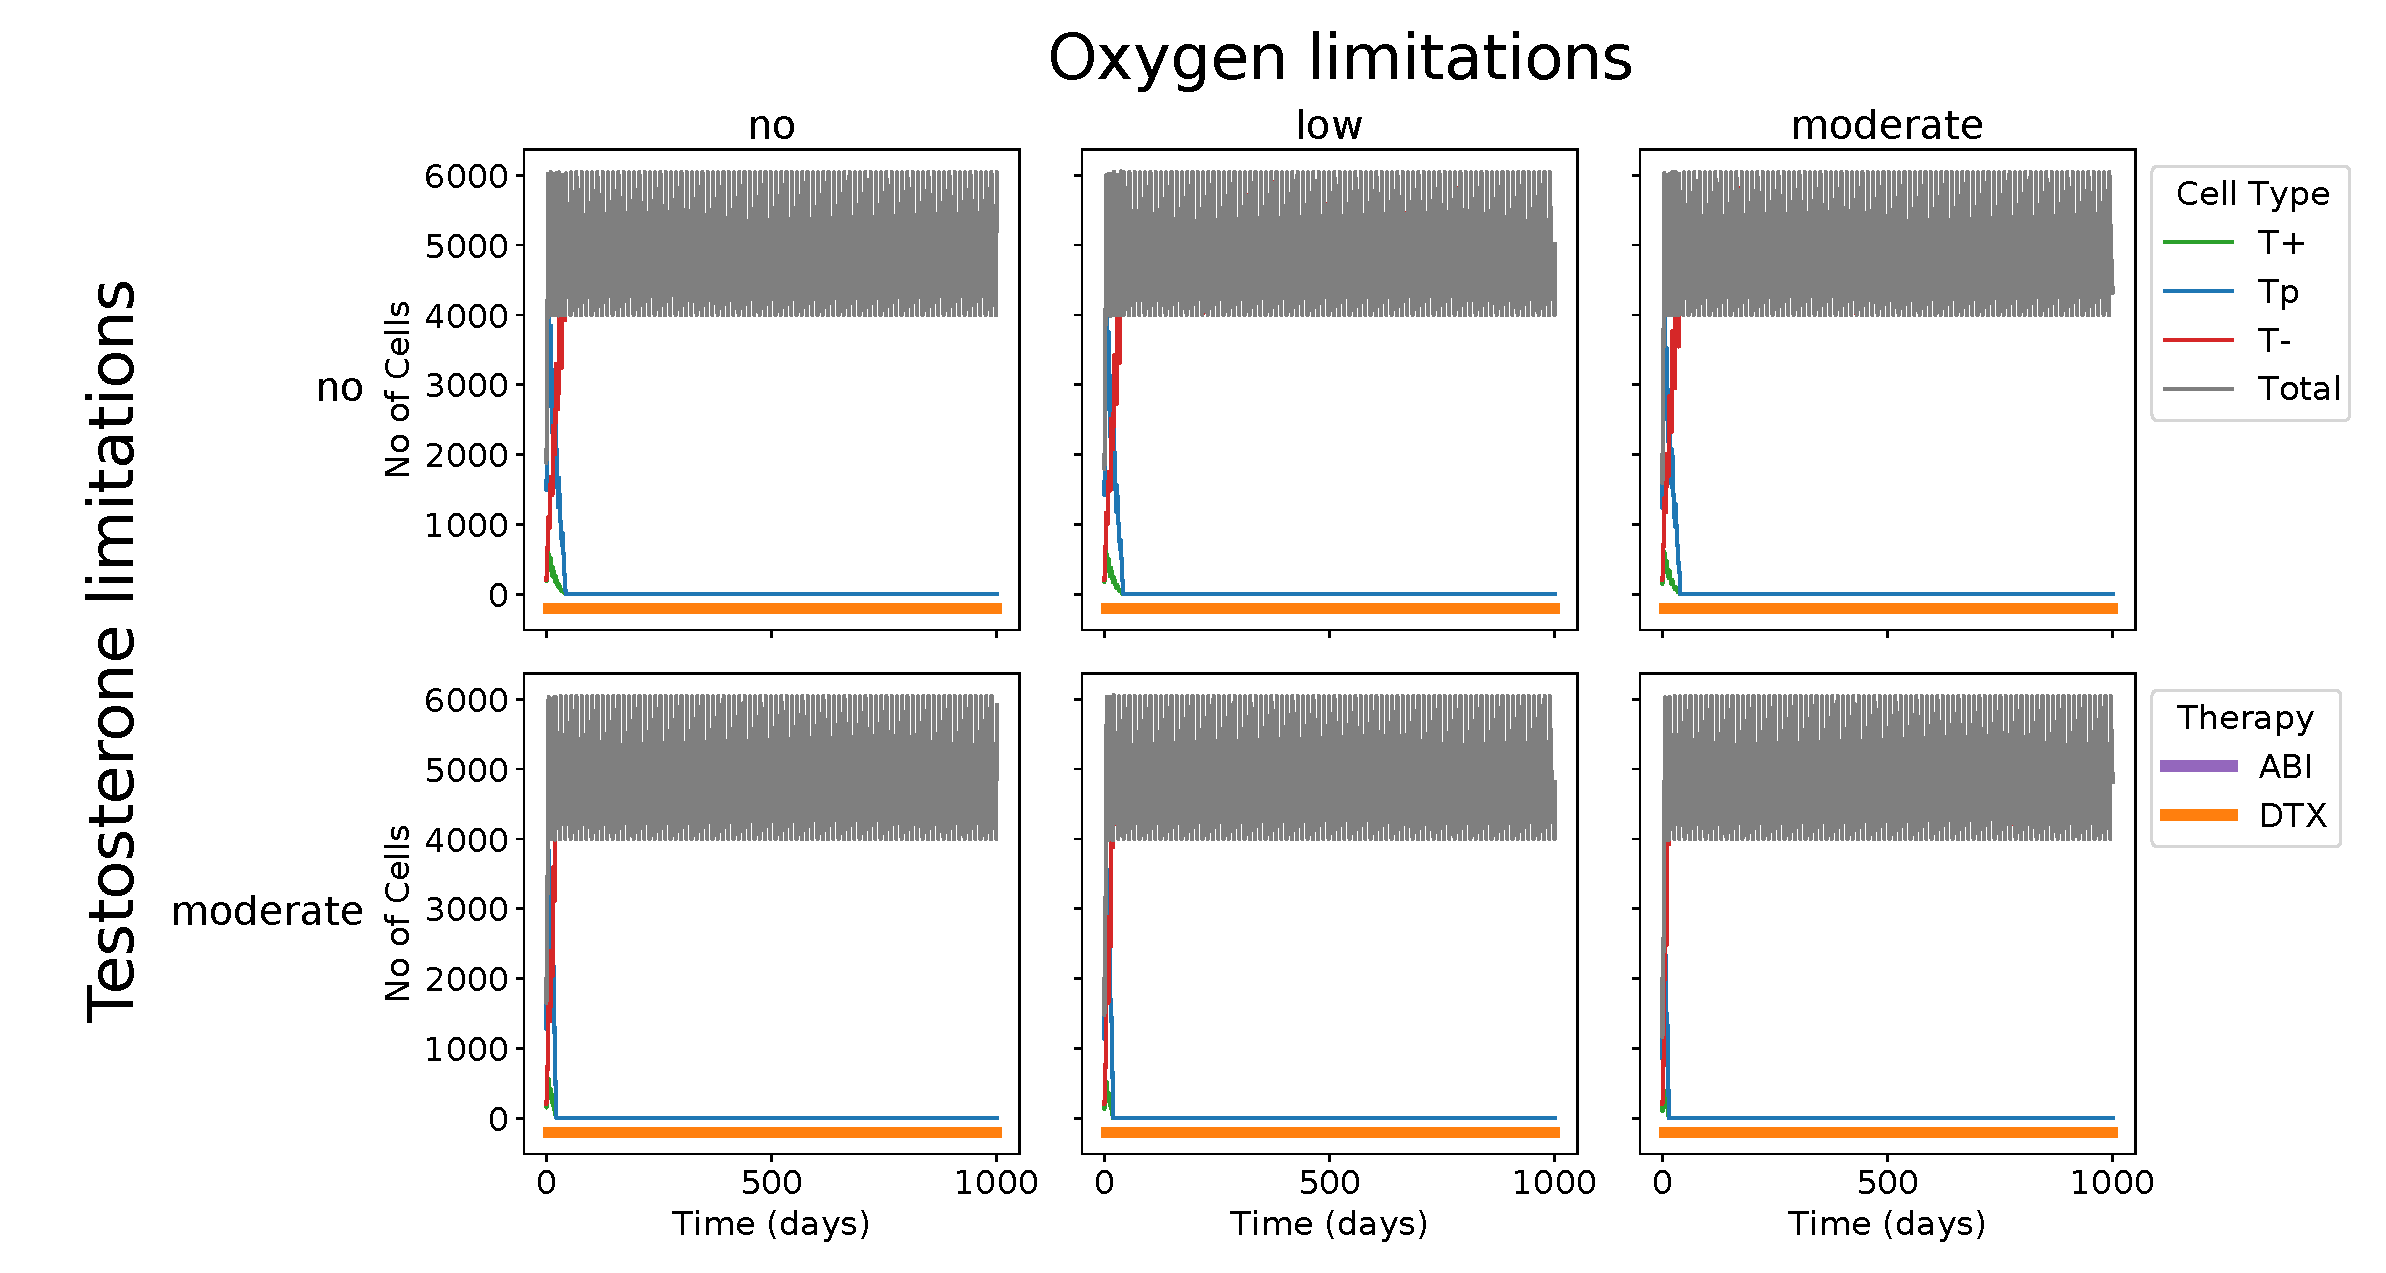
\includegraphics[width=\textwidth]{All3_therapy-combi_8:1:1}
      \caption{High $T^p$ seeding - 8:1:1}
    \end{subfigure}
    \caption{Time-series of all cell types with combination AT of abi and dtx. C: $O_2$ limits, R: $test$ limits and SF: seeding propn. abi(On:6000, Off:4000; $T^+ + T^p$), dtx(On:6000, Off:4000; $T^+ + T^p + T^-$)}
  \end{figure}
  \begin{columns}
    \begin{column}{0.5\textwidth}
      \begin{itemize}
        \item Hormone-specific + cytoxic \cite{West}
        \item Test-of-concept: abi - $T^+ - T^p$, dtx - total
      \end{itemize}
    \end{column}
    \begin{column}{0.5\textwidth}
      \begin{itemize}
        \item $-ve$ effect on $T^+ - T^p$ vs $+ve$ effect $\downarrow$ $T^-$
      \end{itemize}
    \end{column}
  \end{columns}
\end{frame}
